\documentclass[12pt]{beamer}
\usepackage{cmap}
\usepackage[T2A]{fontenc}
\usepackage[utf8]{inputenc}
\usepackage{ifluatex}
\usefonttheme[onlymath]{serif}
\usepackage{svg}
\usepackage{enumerate}
\usepackage{hyperref}
\usepackage{mathtools}
\setbeamertemplate{footline}[frame number]
\definecolor{beamer@darkgreen}{rgb}{0,0.6,0}
\setbeamercolor{normal text}{fg=black,bg=white}
\setbeamercolor{title}{fg=black,bg=beamer@darkgreen}
\setbeamercolor{frametitle}{fg=black,bg=beamer@darkgreen}
\setbeamercolor{background canvas}{parent=normal text}

\usepackage[english,russian]{babel}
\usepackage{graphicx}
\usepackage{listings}
\DeclareMathOperator{\sign}{sign}

\usepackage{enumerate}

\author{Катя Тузова}
\title{Машинное обучение}
\date{}

\subtitle{Лекция 3. Методы кластеризации}

\begin{document}
\frame{\titlepage}


\begin{frame}\frametitle{Разбор летучки}
	Что такое прецедент?
\end{frame}

\begin{frame}\frametitle{Разбор летучки}
	Задача обучения с учителем.\\
	\vspace{5mm}
	Множество объектов $X$ \\
	Множество допустимых ответов $Y$\\
	Прецедент - пара объект-ответ ${(x_i,y_i)}$  \\
	$x_i \in X$ 	$y_i \in Y$
\end{frame}

\begin{frame}\frametitle{Разбор летучки}
	К какому типу задач относятся:
	\begin{itemize}
		\item[--] Прогнозирования потребительского спроса. У компании есть 1000 продуктов, которые она производит. Требуется предсказать сколько будет продано в следующие полгода.
		% регрессия
		\item[--] Вы владелец фейсбука и пишете алгоритм, который определяет был ли взломан пользователь. 
		% классификация
		\item[--] В задачах медицинской диагностики в роли объектов выступают пациенты. Найти вид заболевания.
		%классификация
		\item[--] Задача кредитного скоринга (Оценка кредитоспособности клиента, на основании которой принимается решение о выдаче кредита)
		% классификация
	\end{itemize}
\end{frame}

\begin{frame}\frametitle{Разбор летучки}
	К какому типу задач относятся:
	\begin{itemize}
		\item[--] Прогнозирования потребительского спроса. 
\textcolor{red}{(регрессия)}
		\item[--] Взломан ли пользователь. \textcolor{red}{(бинарная классификация)}
		\item[--] Найти вид заболевания. \textcolor{red}{(классификация)}
		\item[--] Задача кредитного скоринга.  \textcolor{red}{(классификация)}
	\end{itemize}
\end{frame}

\begin{frame}\frametitle{Разбор летучки}
Какие из следующих задач являются задачей обучения без учителя?
\begin{itemize}
	\item[--] Спам фильтр
	\item[--] Рубрикация текстов (Группировка статей по темам)
	\item[--] Оценить есть ли у нового пациента диабет
	\item[--] Прогнозирование времени следующего землетрясения на определенной территории.
	\item[--] Разделение людей по психотипу. 
\end{itemize}
\end{frame}

\begin{frame}\frametitle{Разбор летучки}
Какие из следующих задач являются задачей обучения без учителя?
\begin{itemize}
	\item[--] Спам фильтр
	\item[+] Рубрикация текстов (Группировка статей по темам)
	\item[--] Оценить есть ли у нового пациента диабет
	\item[--] Прогнозирование времени следующего землетрясения на определенной территории.
	\item[+] Разделение людей по психотипу. 
\end{itemize}
\end{frame}

\begin{frame}\frametitle{Разбор летучки}
\begin{itemize}
\item[--] Пол
\item[--] Средний школьный балл
\item[--] Номер школы
\item[--] Город школы
\item[--] Доля пропущенных лекций
\item[--] Оценка по мнению родителей
\item[--] Пиво/неделя
\item[--] Друзей в ВКонтакте
\item[--] Расстояние от дома до универа
\item[--] Ряд в аудитории
\item[--] Наличие планшета
\item[--] Периметр головы
\end{itemize}
\end{frame}

\begin{frame}\frametitle{Разбор летучки}
\begin{itemize}
\item[--] Пол \textcolor{red}{(бинарный)}
\item[--] Средний школьный балл \textcolor{red}{(количественный)}
\item[--] Номер школы \textcolor{red}{(номинальный)}
\item[--] Город школы  \textcolor{red}{(номинальный)}
\item[--] Доля пропущенных лекций   \textcolor{red}{(количественный)}
\item[--] Оценка по мнению родителей   \textcolor{red}{(порядковый)}
\item[--] Пиво/неделя    \textcolor{red}{(количественный)}
\item[--] Друзей в ВКонтакте   \textcolor{red}{(количественный)}
\item[--] Расстояние от дома до универа  \textcolor{red}{(количественный)}
\item[--] Ряд в аудитории  \textcolor{red}{(порядковый)}
\item[--] Наличие планшета  \textcolor{red}{(бинарный)}
\item[--] Периметр головы   \textcolor{red}{(количественный)}
\end{itemize}
\end{frame}

\begin{frame}\frametitle{Разбор летучки}
Приведите пример переобучения и недообучения.
\end{frame}

\begin{frame}\frametitle{Разбор летучки}
Приведите пример переобучения и недообучения.
\begin{figure}[htbp]
  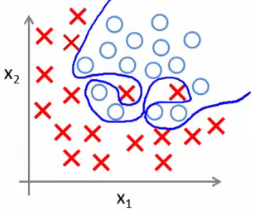
\includegraphics[height=100pt, keepaspectratio = true]{images/overfitting}  
  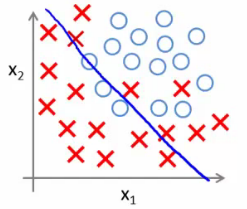
\includegraphics[height=100pt, keepaspectratio = true]{images/underfitting}  
\end{figure}
\end{frame}

\begin{frame}\frametitle{Разбор летучки 2}
Что такое k-fold cross validation? 
\end{frame}

\begin{frame}\frametitle{Разбор летучки 2}
Что такое k-fold cross validation? \\
\vspace{5mm}
Способ разбиения обучающей выборки на два множества $L$ и $T$.\\
$X$ разбивается на $k$ частей. Затем на ${k-1}$ частях данных производится обучение модели, а оставшаяся часть данных используется для тестирования.
\end{frame}

\begin{frame}\frametitle{Разбор летучки 2}
      Что отложено по оси ординат? \\
   \begin{minipage}[t]{0.35\linewidth}

	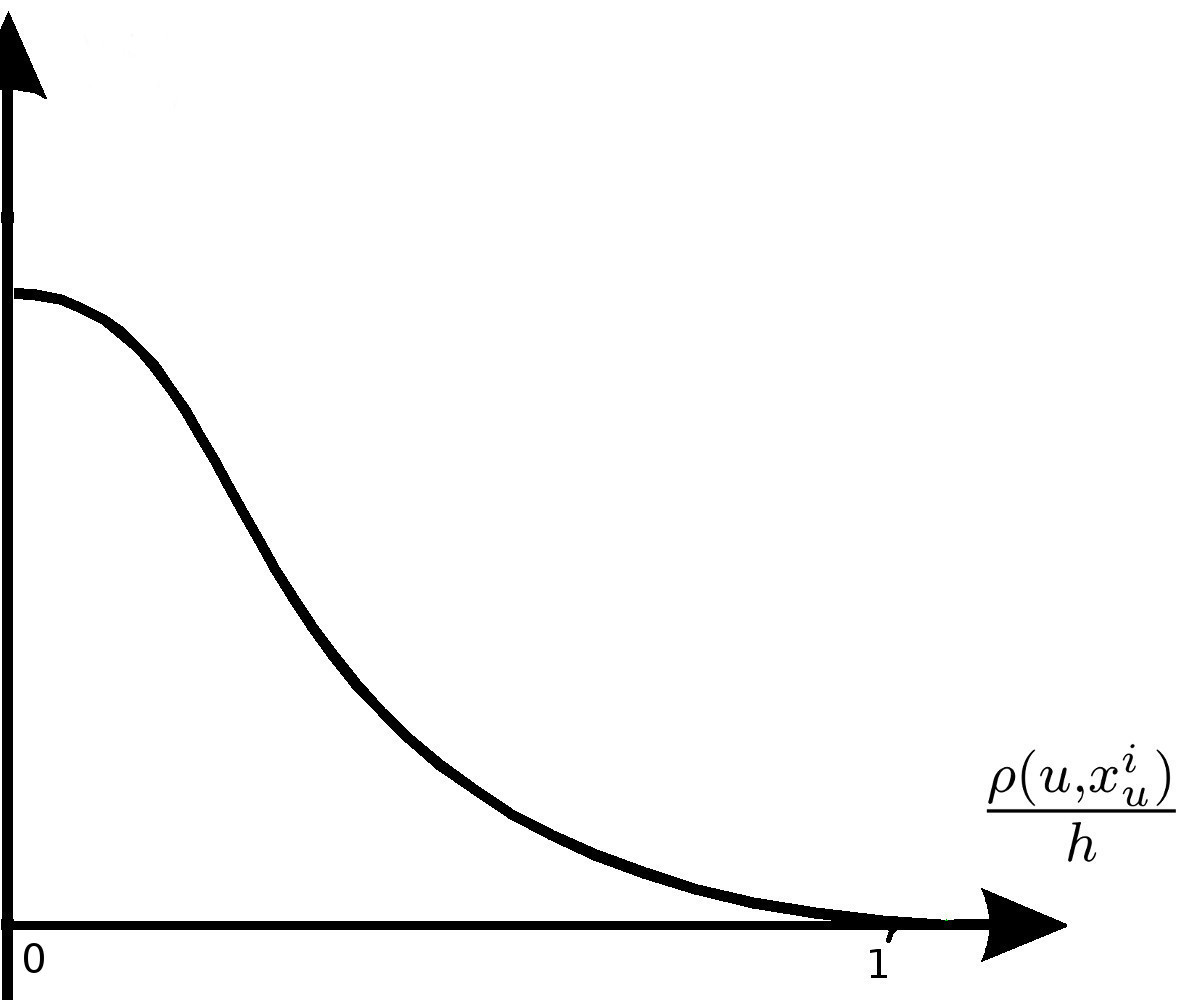
\includegraphics[height=150px]{images/parzen}
   \end{minipage}
\end{frame}

\begin{frame}\frametitle{Разбор летучки 2}
      Что отложено по оси ординат? \\
   \begin{minipage}[t]{0.35\linewidth}

	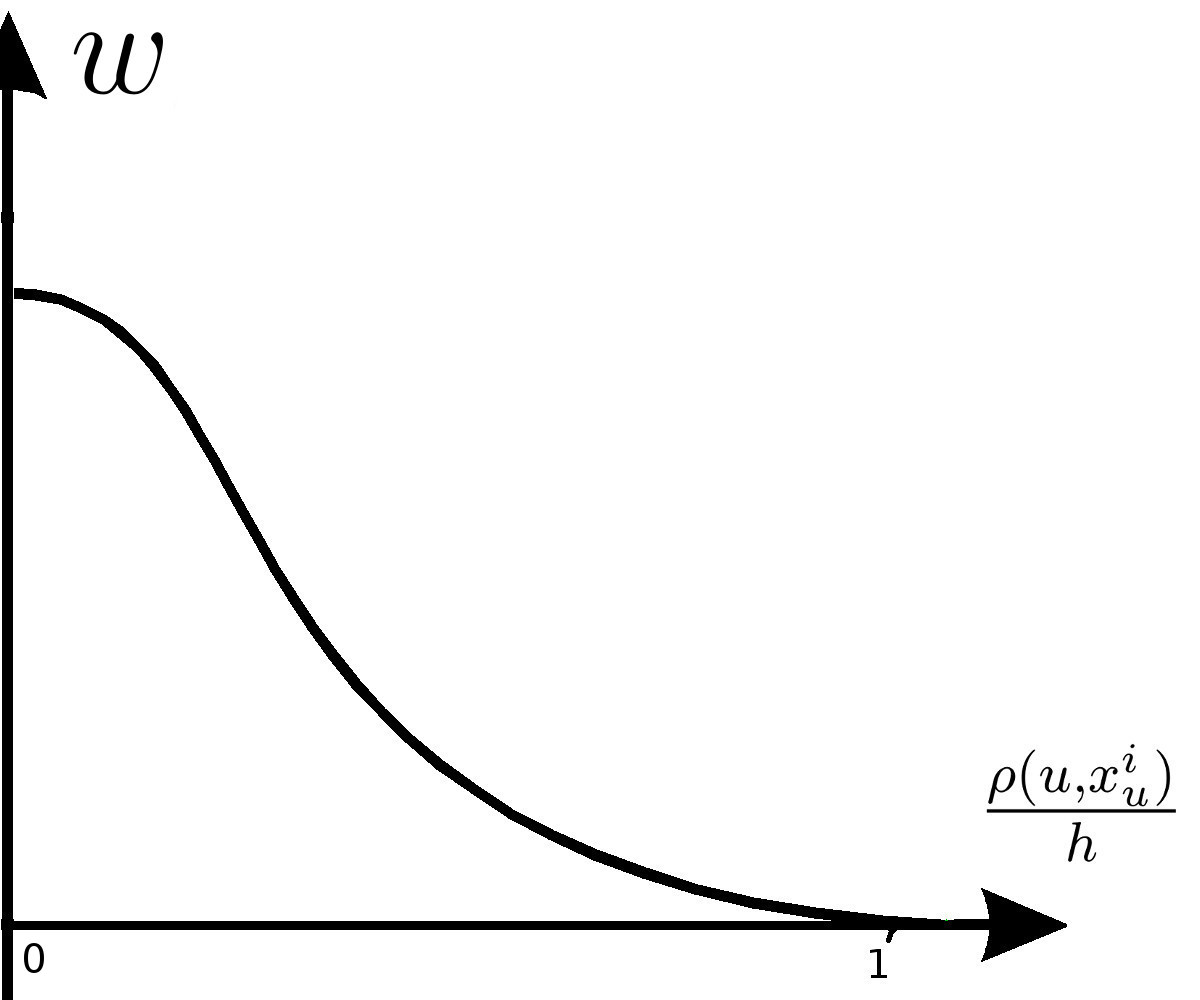
\includegraphics[height=150px]{images/parzen1}
   \end{minipage}
\end{frame}

\begin{frame}\frametitle{Разбор летучки 2}
Чем эталонный объект отличается от надежно классифицируемого?\\
\end{frame}

\begin{frame}\frametitle{Разбор летучки 2}
Чем эталонный объект отличается от надежно классифицируемого?\\
\vspace{8mm}
Эталонные объекты имеют большой положительный отступ, плотно окружены
объектами своего класса и являются наиболее типичными его представителями.\\
\vspace{5mm}
Надежно классифицируемые(неинформативные) объекты -- изъятие
этих объектов из выборки не влияет на качество классификации. Фактически, они не добавляют к эталонам никакой новой информации. 

\end{frame}


\begin{frame}\frametitle{Разбор летучки 2}
${a(u, X^l) = \arg\max\limits_{y \in Y} \underbrace{\sum\limits_{i=1}^l [y_u^i = y]w(i, u)}_{\Gamma_y(u)} }$\\
Смысл параметров $w$, $i$, $u$, $\Gamma_y(u)$
\end{frame}

\begin{frame}\frametitle{Разбор летучки 2}
${a(u, X^l) = \arg\max\limits_{y \in Y} \underbrace{\sum\limits_{i=1}^l [y_u^i = y]w(i, u)}_{\Gamma_y(u)} }$\\
$w(i, u)$ - вес $i$-го соседа $u$ \\
$i$ - порядковый номер соседа $u$ в упорядоченном множестве\\
$u$ -- объект, для которого проводится классификация\\
$\Gamma_y(u)$ -- оценка близости объекта $u$ к классу ${y}$
\end{frame}

\begin{frame}\frametitle{Разбор летучки 2}
Мотивация для использования Парзеновского окна. В чем минусы зависимости веса объекта только от его порядкового номера?
\end{frame}

\begin{frame}\frametitle{Разбор летучки 2}
Мотивация для использования Парзеновского окна. В чем минусы зависимости веса объекта только от его порядкового номера?\\
\vspace{5mm}
Объекты, находящиеся на одинаковом расстоянии будут взяты с разными весами. 
Далекие объекты могут быть взяты со слишком большим весом.
\end{frame}

\begin{frame}\frametitle{Разбор летучки 2}
\textbf{Гипотеза компактности:}\\
Схожие объекты, как правило, лежат в одном классе.\\
\end{frame}

\begin{frame}\frametitle{Разбор летучки 2}
Какие проблемы могут встретиться при использовании метода k-nn на реальных
данных? Какие решения этих проблем вам известны?
\end{frame}

\begin{frame}\frametitle{Разбор летучки 2}
Какие проблемы могут встретиться при использовании метода k-nn на реальных
данных? Какие решения этих проблем вам известны?\\
\vspace{5mm}
\begin{itemize}
\item[--] Разные шкалы признаков
\item[--] Проблема подбора метрики
\item[--] Проклятие размерности
\item[--] Хранение выборки
\item[--] Быстрый поиск ближайших соседей
\end{itemize}
\end{frame}


\begin{frame}\frametitle{Разбор летучки 2}
Какими свойствами должна обладать функция $K$, чтобы использовать ее в качестве ядра?
\end{frame}

\begin{frame}\frametitle{Разбор летучки 2}
Какими свойствами должна обладать функция $K$, чтобы использовать ее в качестве ядра?\\
\vspace{5mm}
Невозрастающая функция, положительная на отрезке [0, 1]
\end{frame}


\begin{frame}\frametitle{Общие вопросы по домашке}

$$\operatorname{Precision} = \frac{TP}{TP + FP}
\qquad
\operatorname{Recall} = \frac{TP}{TP + FN}$$
\begin{itemize}
\item[--] $TP$ --- это количество элементов, которые классификатор верно отнёс к классу $c$,
\item[--] $FP$ --- количество элементов, которые классификатор неверно отнёс к классу $c$,
\item[--] $FN$ --- количество элементов, которые классификатор неверно отнёс к классу, отличному от $c$.
\end{itemize}
\end{frame}

\begin{frame}\frametitle{Общие вопросы по домашке}
\begin{itemize}
\item[--] Нужна ли нормировка признаков?
\item[--] В чем минус поиска ближайших соседей с помощью сортировки?
\end{itemize}
\end{frame}

\begin{frame}\frametitle{Общие вопросы по домашке}
\begin{figure}[htbp]
  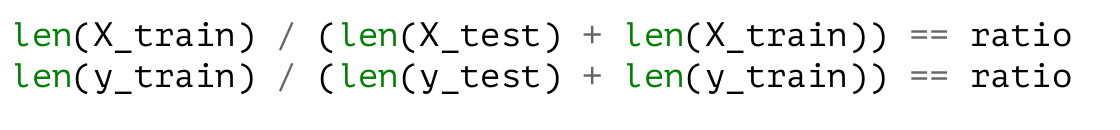
\includegraphics[height=35pt, keepaspectratio = true]{images/hw}  
\end{figure}

\vspace{5mm}
Как выбрать ratio?
\end{frame}

\begin{frame}\frametitle{Общие вопросы по домашке}
\begin{itemize}
\item[--] Надо ли было брать $k = 1$ в функции loocv?
\item[--] Можно ли не перебирать $k$ от $1$ до $n$?
\item[--] Можно ли остановиться при выборе $k$ как только начнет увеличиваться LOO?
\item[--] Надо ли было использовать тестовые данные в функции loocv?
\end{itemize}
\end{frame}

\begin{frame}\frametitle{Пример зависимости $k$}
\begin{figure}[htbp]
  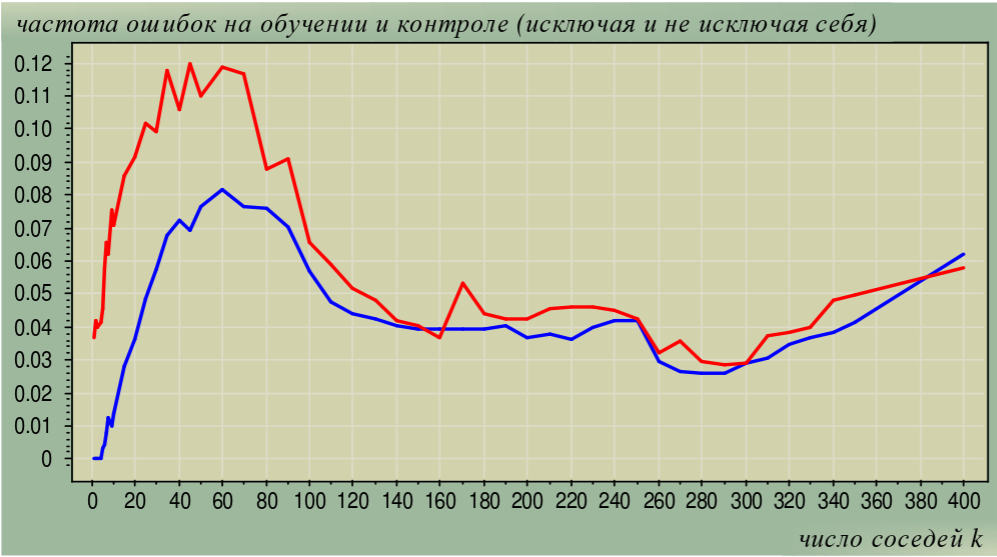
\includegraphics[height=180pt, keepaspectratio = true]{images/breast_cancer}  
\end{figure}
\textcolor{gray}{картинка с machinelearning.ru}
\end{frame}

\begin{frame}\frametitle{Быстрый поиск ближайшего соседа}
\end{frame}

\begin{frame}\frametitle{k-d дерево}
Идея: разложим множество по поторому будем искать
в бинарное дерево с простыми условиями и
конкретными точками в узлах.
\vspace{5mm}
\begin{enumerate}
\item По циклу, или рандомно выбираем ось.
\item Ищем медиану (точку, разбивающую множество на как
можно более равные части).
\item Повторяем 1-2 для каждого из получившихся подмножеств 
\end{enumerate}
Сложность построения: $O(n\log n)$\\
Сложность поиска: в лучшем
случае $O(\log n)$, в худшем -- $O(n)$
\end{frame}
\begin{frame}\frametitle{2-d дерево}

\begin{figure}[htbp]
\centering
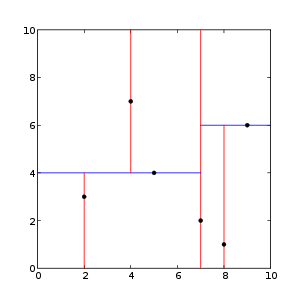
\includegraphics[height=190pt]{images/Kdtree_2d}  
\end{figure}
\end{frame}

\begin{frame}\frametitle{k-d дерево. Особенности}
\begin{itemize}
\item[+] Один из наиболее простых методов
\item[--] Работает только при малом количестве параметров
\item[--] Затратный алгоритм перестроения

\end{itemize}
\end{frame}

\begin{frame}\frametitle{Locality Sensitive Hash}
Задача: Найти похожие документы в интернете\\
\vspace{5mm}
\end{frame}

\begin{frame}\frametitle{Locality Sensitive Hash}
Проблема: Сколько сравнений нам понадобится  для того, чтобы найти похожие среди $N$ документов?\\
\vspace{5mm}
\end{frame}

\begin{frame}\frametitle{Locality Sensitive Hash}
Проблема: Сколько сравнений нам понадобится  для того, чтобы найти похожие среди $N$ документов?\\
\vspace{5mm}
$C = \frac{N(N-1)}{2}$\\
\vspace{5mm}
$N = 10^6 \Rightarrow C = 5*10^{11}$
\end{frame}

\begin{frame}\frametitle{Locality Sensitive Hash}
Идея:\\
Давайте от каждого документа (строки из нулей и единиц) возьмем хэш $h$:\\
\begin{itemize}
\item[--] Если документы $C_1$ и $C_2$ похожи, то с большой вероятностью $h(C1) == h(C2)$\\
\item[--] Иначе -- с большой вероятностью $h(C1) \neq h(C2)$
\end{itemize}
\end{frame}

\begin{frame}\frametitle{Locality Sensitive Hash}
Идея: \\
\begin{itemize}
\item[--] Разбить документ на n-граммы
\item[--] Взять от каждого n-грамма хэш
\item[--] Получим представление документа в виде строки из нулей и единиц. Длина такого вектора = количество всевозможных n-грамм.
\item[--] Посчитаем документы похожими, если у них много совпадающих n-грамм
\end{itemize}
\end{frame}

\begin{frame}\frametitle{Locality Sensitive Hash}
\begin{figure}[htbp]
\centering
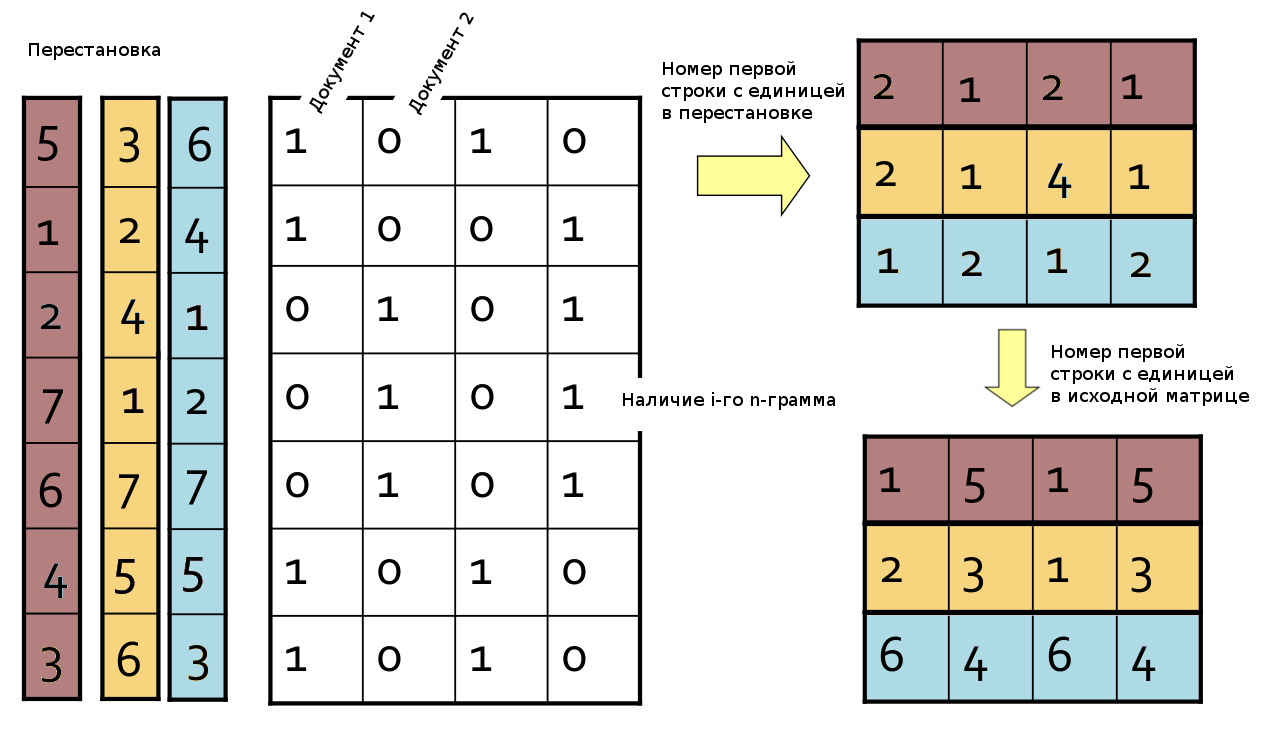
\includegraphics[height=190pt]{images/min-hash1}  
\end{figure}
\end{frame}

\begin{frame}\frametitle{Задача кластеризации}
\end{frame}

\begin{frame}\frametitle{Постановка задачи кластеризации}
Кластеризация -- задача разделения объектов одной природы на несколько групп так, чтобы объекты в одной группе обладали одним и тем же свойством.\\
\vspace{5mm}
Кластеризация -- это обучение без учителя.
\end{frame}

\begin{frame}\frametitle{Постановка задачи кластеризации}
$X$ -- пространство объектов\\
$\rho: X \times X \rightarrow [0, \infty)$ -- функция расстояния между объектами\\
\vspace{5mm}
Найти:\\
$Y$ -- множество кластеров \\
$a: X \rightarrow Y$ -- алгоритм кластеризации
\vspace{5mm}

\end{frame}

\begin{frame}\frametitle{Степени свободы в постановке задачи}
\end{frame}

\begin{frame}\frametitle{Степени свободы в постановке задачи}
	\begin{itemize}
		\item[--] Критерий качества кластеризации
		\item[--] Число кластеров неизвестно заранее
		\item[--] Результат кластеризации существенно зависит от метрики
	\end{itemize}
\end{frame}

\begin{frame}\frametitle{Цели кластеризации}
\end{frame}

\begin{frame}\frametitle{Цели кластеризации}
	\begin{itemize}
		\item[--] Сократить объём хранимых данных
		\item[--] Выделить нетипичные объекты
		\item[--] Упростить дальнейшую обработку данных
		\item[--] Построить иерархию множества объектов				
	\end{itemize}
\end{frame}

\begin{frame}\frametitle{Какие бывают кластеры?}
\end{frame}

\begin{frame}\frametitle{Типы кластерных структур. Сгущения}
\begin{figure}[htbp]
  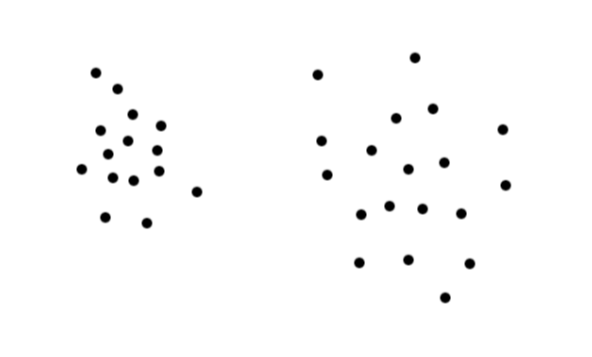
\includegraphics[height=130pt, keepaspectratio = true]{images/cluster1}  
\end{figure}
\end{frame}

\begin{frame}\frametitle{Типы кластерных структур. Ленты}
\begin{figure}[htbp]
  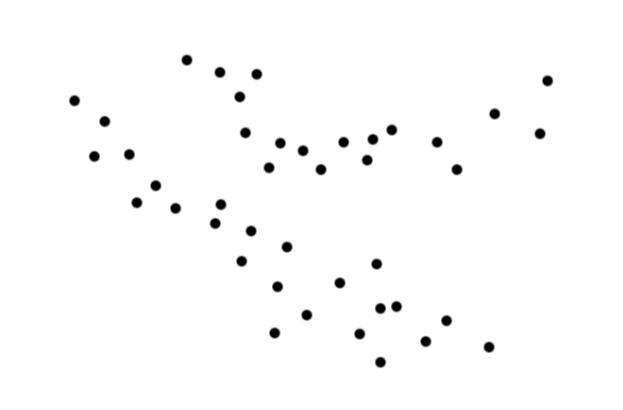
\includegraphics[height=130pt, keepaspectratio = true]{images/cluster2}  
\end{figure}
\end{frame}

\begin{frame}\frametitle{Типы кластерных структур. С центром}
\begin{figure}[htbp]
  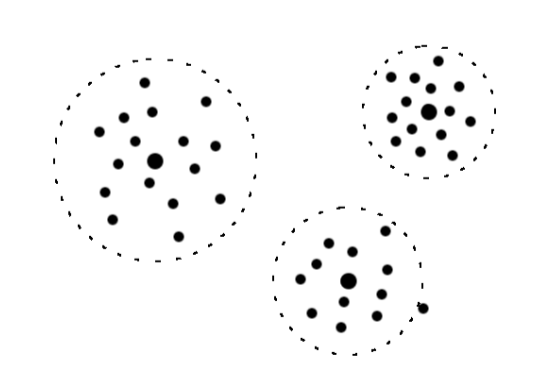
\includegraphics[height=130pt, keepaspectratio = true]{images/cluster3}  
\end{figure}
\end{frame}

\begin{frame}\frametitle{Типы кластерных структур. С перемычками}
\begin{figure}[htbp]
  
\includegraphics[height=130pt, keepaspectratio = true]{images/cluster4}  
\end{figure}
\end{frame}

\begin{frame}\frametitle{Типы кластерных структур. На фоне}
\begin{figure}[htbp]
  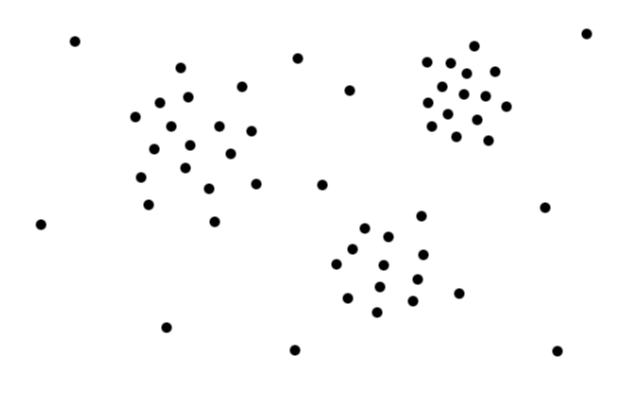
\includegraphics[height=130pt, keepaspectratio = true]{images/cluster5}  
\end{figure}
\end{frame}

\begin{frame}\frametitle{Типы кластерных структур. Перекрывающиеся}
\begin{figure}[htbp]
  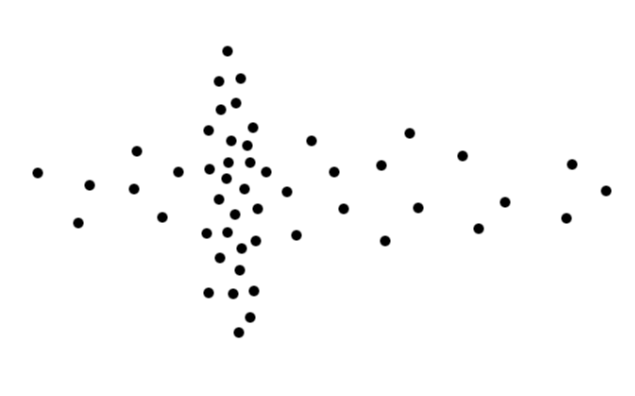
\includegraphics[height=130pt, keepaspectratio = true]{images/cluster6}  
\end{figure}
\end{frame}

\begin{frame}\frametitle{Чувствительность к выбору метрики}
\begin{figure}[htbp]
  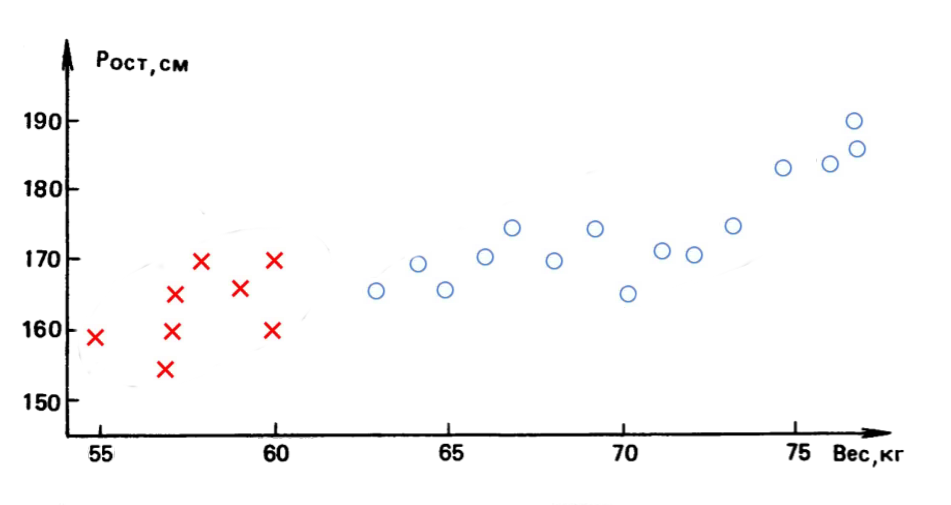
\includegraphics[height=160pt, keepaspectratio = true]{images/students}  
\end{figure}
\end{frame}

\begin{frame}\frametitle{Чувствительность к выбору метрики}
\begin{figure}[htbp]
  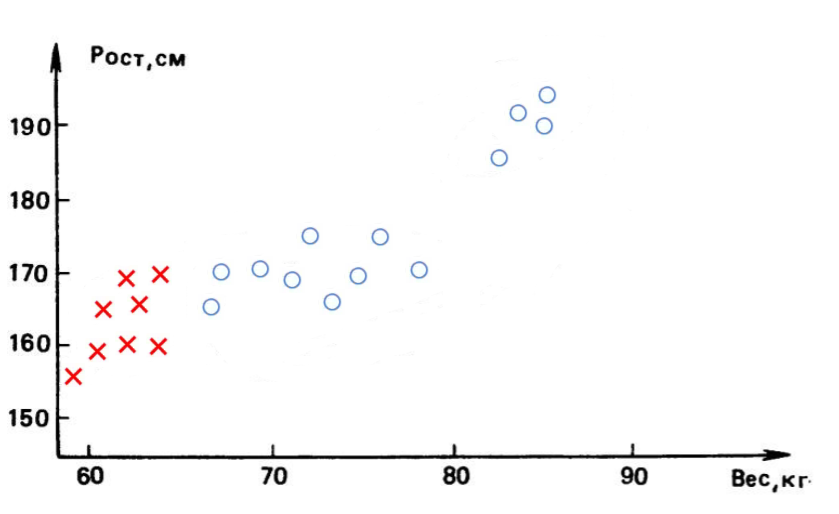
\includegraphics[height=160pt, keepaspectratio = true]{images/students1}  
\end{figure}
\end{frame}

\begin{frame}\frametitle{Чувствительность к выбору метрики}
\begin{figure}[htbp]
  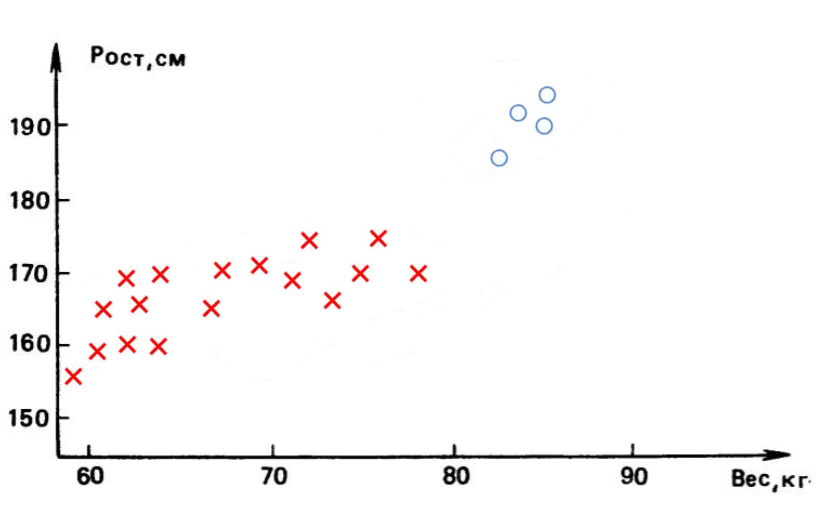
\includegraphics[height=160pt, keepaspectratio = true]{images/students2}  
\end{figure}
\end{frame}

\begin{frame}\frametitle{Оценка качества кластеризации}
Есть несколько разбиений на кластеры. Как их сравнить?
\end{frame}

\begin{frame}\frametitle{Оценка качества кластеризации}
\begin{itemize}
\item[--] Минимизировать среднее внутрикластерное расстояние\\
\vspace{5mm}
${\frac{\sum\limits_{a(x_i) = a(x_j)} \rho(x_i, x_j)}{\sum\limits_{a(x_i) = a(x_j)} 1} \rightarrow \min}$
\item[--] Максимизировать среднее межкластерное расстояние\\
\vspace{5mm}
${\frac{\sum\limits_{a(x_i) \neq a(x_j)} \rho(x_i, x_j)}{\sum\limits_{a(x_i) \neq a(x_j)} 1} \rightarrow \max}$
\end{itemize}
\end{frame}

\begin{frame}\frametitle{Методы кластеризации}
\begin{itemize}
\item[--] Иерархические
\item[--] Графовые 
\item[--] Статистические 
\end{itemize}
\end{frame}

\begin{frame}\frametitle{Иерархическая кластеризация}
\end{frame}

\begin{frame}\frametitle{Агломеративный алгоритм Ланса-Уильямса}
Идея:\\
\begin{itemize}
\item[--] Считаем каждую точку кластером. 
\item[--] Затем объединяем ближайшие точки в новый кластер. 
\item[--] Повторяем.
\end{itemize}
\end{frame}


\begin{frame}\frametitle{Алгоритм Ланса-Уильямса}

${C_1 = \left\{ \left\{ x_1\right\}, \left\{x_2 \right\}, \dots, \left\{x_l \right\} \right\}}$\\
for ${t=2, \dots, l }$:\\
\hspace{5mm} ${(U, V) = \arg\min\limits_{U \neq V} \rho(U, V)}$\\
\hspace{5mm} $W = U \cup V$\\
\hspace{5mm} ${C_t = C_{t-1} \cup \left\{ W \right\}\setminus \left\{U, V \right\} }$\\
\hspace{5mm} foreach ${S \in C_t}$\\
\hspace{10mm}   вычислить $\rho(W, S)$\\

\end{frame}


\begin{frame}\frametitle{Алгоритм Ланса-Уильямса}
Чего не хватает?
\end{frame}

\begin{frame}\frametitle{Формула Ланса-Уильямса}
\begin{minipage}[t]{0.55\linewidth}
Расстояние $\rho(W, S)$?\\
${ W = \left\{ U \cup V \right\} }$\\

Знаем:\\
${\rho(U, S), \rho(V, S), \rho(U, V)}$

\end{minipage}%
\begin{minipage}[t]{0.45\linewidth}
    \begin{figure}[htbp]
  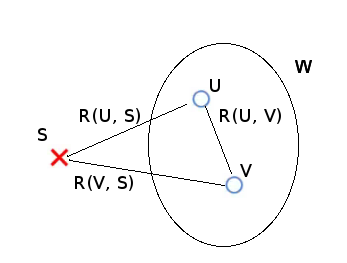
\includegraphics[height=130pt, keepaspectratio = true]{images/lans-formula}  
\end{figure}
\end{minipage}%

\end{frame}

\begin{frame}\frametitle{Формула Ланса-Уильямса}
Расстояние $\rho(W, S)$?\\
${ W = \left\{ U \cup V \right\} }$\\
\vspace{5mm}
Знаем:\\
${\rho(U, S), \rho(V, S), \rho(U, V)}$\\
\vspace{5mm}
${\rho(U \cup V, S) = \alpha_U \rho(U, S) + \alpha_V \rho(V, S) + }$ \\
\hspace{30mm} ${ + \beta \rho(U, V) + \gamma \vert \rho(U, S) - \rho(V, S)\vert}$\\
\vspace{5mm}
${\alpha_U, \alpha_V, \beta, \gamma}$ -- числовые параметры
\end{frame}

\begin{frame}\frametitle{Формула Ланса-Уильямса}
Значения параметров
${\alpha_U, \alpha_V, \beta, \gamma}$ ?
\end{frame}

\begin{frame}\frametitle{Формула Ланса-Уильямса}
Расстояние ближнего соседа:\\
\begin{figure}[htbp]
  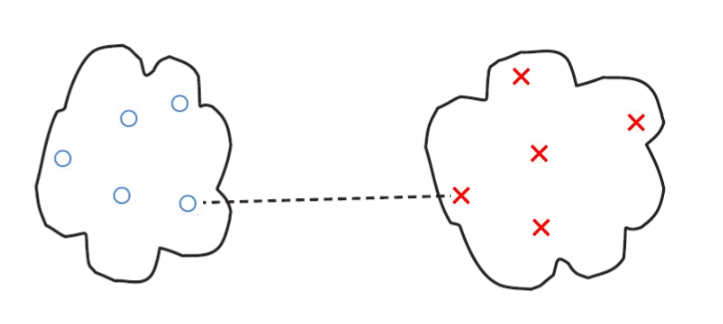
\includegraphics[height=100pt, keepaspectratio = true]{images/lans1}  
\end{figure}
\end{frame}

\begin{frame}\frametitle{Формула Ланса-Уильямса}
Расстояние ближнего соседа:\\
\begin{figure}[htbp]
  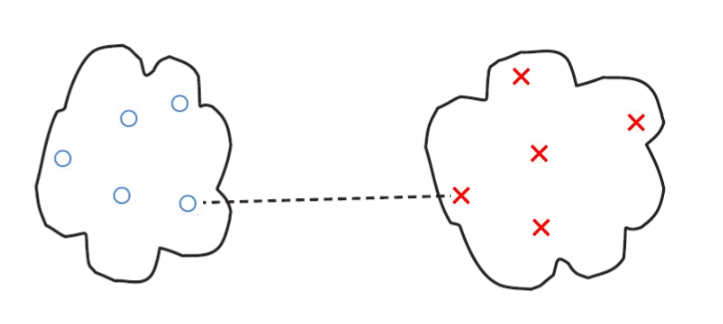
\includegraphics[height=100pt, keepaspectratio = true]{images/lans1}  
\end{figure}
${\alpha_U = \alpha_V = \frac{1}{2}}$ \\${\beta = 0}$ \\${\gamma = -\frac{1}{2}}$
\end{frame}

\begin{frame}\frametitle{Формула Ланса-Уильямса}
Расстояние дальнего соседа:\\
\begin{figure}[htbp]
  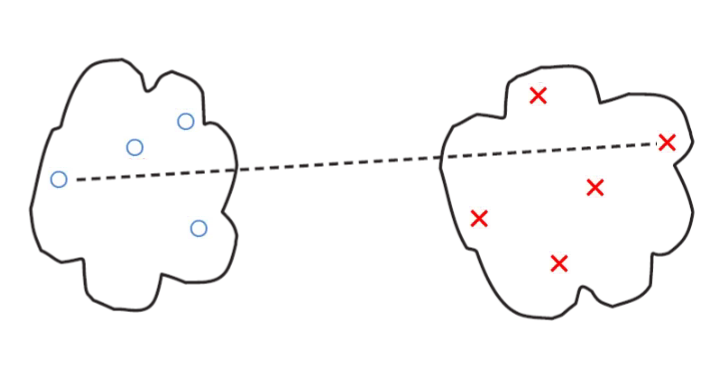
\includegraphics[height=100pt, keepaspectratio = true]{images/lans2}  
\end{figure}
\end{frame}

\begin{frame}\frametitle{Формула Ланса-Уильямса}
Расстояние дальнего соседа:\\
\begin{figure}[htbp]
  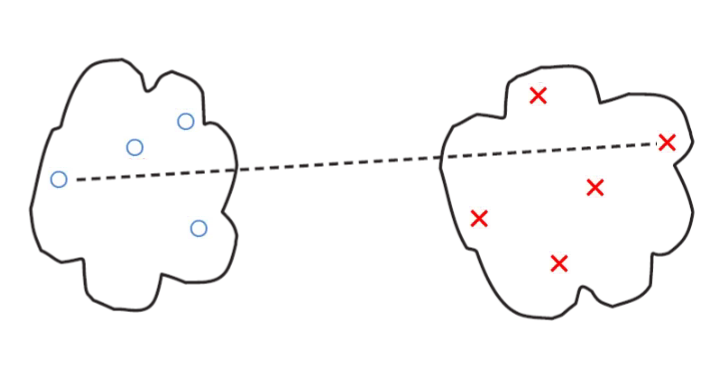
\includegraphics[height=100pt, keepaspectratio = true]{images/lans2}  
\end{figure}
${\alpha_U = \alpha_V = \frac{1}{2}}$ \\${\beta = 0}$ \\${\gamma = \frac{1}{2}}$
\end{frame}

\begin{frame}\frametitle{Формула Ланса-Уильямса}
Групповое среднее:\\
\begin{figure}[htbp]
  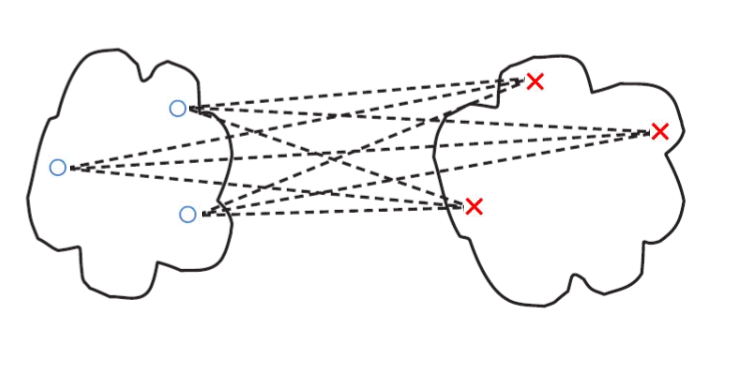
\includegraphics[height=100pt, keepaspectratio = true]{images/lans3}  
\end{figure}
\end{frame}

\begin{frame}\frametitle{Формула Ланса-Уильямса}
Групповое среднее:\\
\begin{figure}[htbp]
  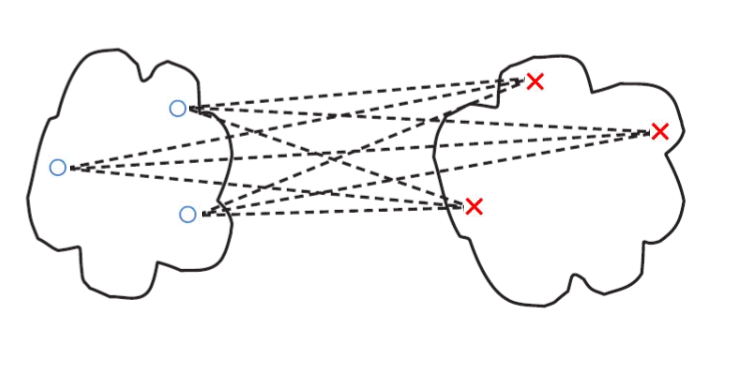
\includegraphics[height=100pt, keepaspectratio = true]{images/lans3}  
\end{figure}
${\alpha_U = \frac{\vert U \vert}{\vert W \vert}}$\\${\alpha_V = \frac{\vert V \vert}{\vert W \vert}}$ \\${\beta = \gamma = 0}$
\end{frame}

\begin{frame}\frametitle{Формула Ланса-Уильямса}
Расстояние Уорда:\\
\begin{figure}[htbp]
  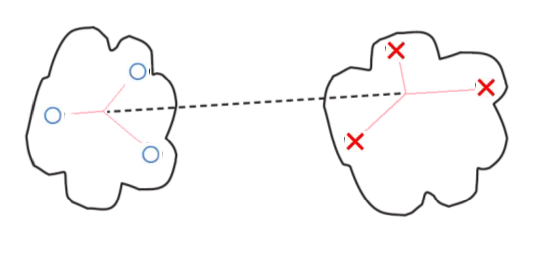
\includegraphics[height=100pt, keepaspectratio = true]{images/lans4}  
\end{figure}

${\alpha_U = \frac{\vert S \vert + \vert U \vert}{\vert S \vert + \vert W \vert}}$\\${\alpha_V = \frac{\vert S \vert + \vert V \vert}{\vert S \vert + \vert W \vert}}$ \\${\beta = \frac{ -\vert S \vert}{\vert S \vert + \vert W \vert}}$ \\${\gamma = 0}$
\end{frame}

\begin{frame}\frametitle{Визуализация кластеров}
\end{frame}

\begin{frame}\frametitle{Диаграмма вложения}
\begin{figure}[htbp]
  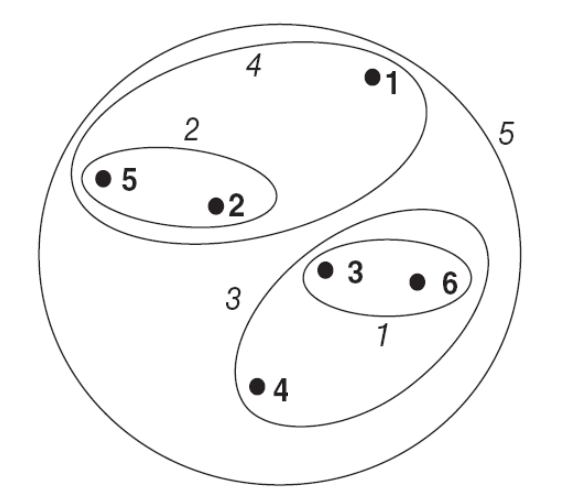
\includegraphics[height=170pt, keepaspectratio = true]{images/diagram}  
\end{figure}
\end{frame}

\begin{frame}\frametitle{Дендрограмма}
\begin{figure}[htbp]
  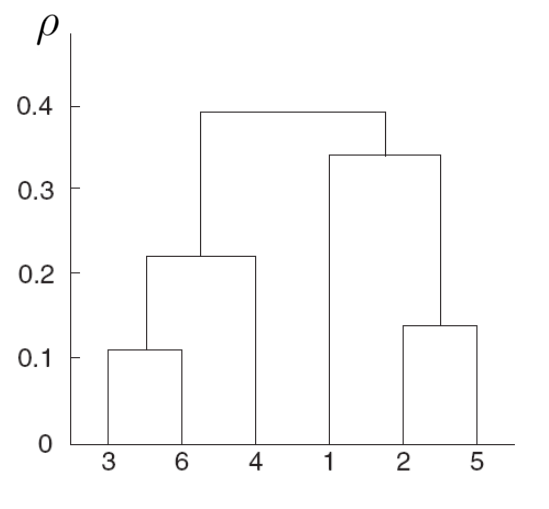
\includegraphics[height=170pt, keepaspectratio = true]{images/dendrogram}  
\end{figure}
\end{frame}

\begin{frame}\frametitle{Дендрограмма}
Может ли так случиться, что дендрограмма имеет самопересечения?
\end{frame}


\begin{frame}\frametitle{Дендрограмма}
Может ли так случиться, что дендрограмма имеет самопересечения?\\
\vspace{5mm}
Как избежать?
\end{frame}

\begin{frame}\frametitle{Свойство монотонности}
Кластеризация монотонна, если на каждом шаге расстояние $\rho$ между объединяемыми кластерами не уменьшается.\\
$\rho_2 \leq \rho_3 \leq \dots \leq \rho_l$
\end{frame}

\begin{frame}\frametitle{На следующей лекции}
\begin{itemize}
\item[--] Задача кластеризации
\item[--] Графовые алгоритмы кластеризации
\item[--] Статистические алгоритмы кластеризации
\end{itemize}
\end{frame}

\end{document}
